\documentclass[UTF8,a4paper,zihao=-4]{ctexart}

\usepackage{geometry}
\usepackage{booktabs}
\usepackage{array}
\usepackage{longtable}
\usepackage{amsmath}
\usepackage{siunitx}
\usepackage{xcolor}
\usepackage{hyperref}
\usepackage{float}
\usepackage{graphicx}
\usepackage{tikz}
\usetikzlibrary{arrows.meta,positioning,fit}

\geometry{left=2.2cm,right=2.2cm,top=2.2cm,bottom=2.4cm}
\hypersetup{colorlinks=true,linkcolor=blue,urlcolor=blue}
\sisetup{detect-all,group-separator={,},group-minimum-digits=4}
\emergencystretch=2em

\title{Lab8 矩阵乘加速器设计报告}
\author{2400011041 徐子翔}
\date{2026 年 6 月 30 日}

\begin{document}
\maketitle

\section{设计目标}

本设计实现 $512\times512$ 的有符号 8 bit 矩阵乘，并输出有符号 32 bit 结果。最终版本以功能正确、低功耗和低延迟为主要目标，并保持单时钟设计。

\section{总体结构}

提交包采用可运行目录结构，主要文件如下：
\begin{itemize}
  \item \texttt{rtl/accelerator\_top.v}：功能仿真顶层，包含 controller、行为级 B SRAM 和计算核实例。
  \item \texttt{rtl/accelerator\_logic\_top.v}：logic-only PPA 综合顶层，只包含计算阵列及其必要门控逻辑。
  \item \texttt{rtl/accelerator\_sram\_ext.v}：PE/MAC 阵列。
  \item \texttt{rtl/sram\_model.v}：pre-syn 功能仿真使用的同步 SRAM 行为模型。
  \item \texttt{testbench/pre-syn}：完整功能仿真并生成 \texttt{result\_mem.csv}。
  \item \texttt{syn/syn.tcl}：Design Compiler logic-only 综合脚本。
\end{itemize}

整体数据流为：controller 从 input memory 读取 A/B 矩阵数据，将当前 B column tile 写入两个 128 bit 行为 SRAM bank；A 矩阵采用 direct-A word buffer，不再额外实例化 A SRAM；计算核执行 $1\times32$ tile 的 dot product 累加；结果经 result memory 接口按 64 bit word 写出。

\section{提交包与运行方式}
\subsection{提交包结构}
提交包根目录包含 RTL、testbench、综合脚本、输入数据、检查脚本、PDK 文件和本报告。主要入口如下：
\begin{itemize}
  \item \texttt{Makefile}：顶层运行入口。
  \item \texttt{input\_mem.csv} 与 \texttt{in.npy}：输入。
  \item \texttt{result\_mem.csv}：pre-syn 的输出结果。
  \item \texttt{CheckResult.py}：结果正确性检查脚本。
  \item \texttt{syn/log/area.rpt}、\texttt{syn/log/power.rpt}、\texttt{syn/log/timing.rpt}：综合结果报告。
  \item \texttt{pdk/NanGate\_15nm\_OCL\_slow\_conditional\_ccs.db}：Design Compiler 使用的 slow corner DB。
  \item \texttt{pdk/NanGate\_15nm\_OCL\_conditional.v}：门级仿真使用的标准单元 Verilog model。
\end{itemize}
\subsection{运行方式}
在支持 make、VCS 或 Icarus、Design Compiler 的环境中，可以在提交包根目录使用以下命令：
\begin{itemize}
  \item \texttt{make}：检查必要文件并运行 pre-syn 功能仿真，不依赖 Python 或 NumPy。
  \item \texttt{make all}：运行 pre-syn 功能仿真、logic-only 综合和后综合 SDF 验证。
  \item \texttt{make generate\_input}：可选命令，用 Python 重新生成输入数据，需要 NumPy。
  \item \texttt{make check\_result}：可选命令，用 Python 检查 \texttt{result\_mem.csv}，需要 NumPy。
\end{itemize}

综合脚本和 testbench 均优先支持完整 NanGate 目录结构；若不存在完整目录，则使用提交包中保留的 flat PDK 文件。因此当前提交包只需上述 DB 和 Verilog model 即可运行本设计流程。

\section{关键设计参数}

\begin{figure}[H]
\centering
\resizebox{\textwidth}{!}{%
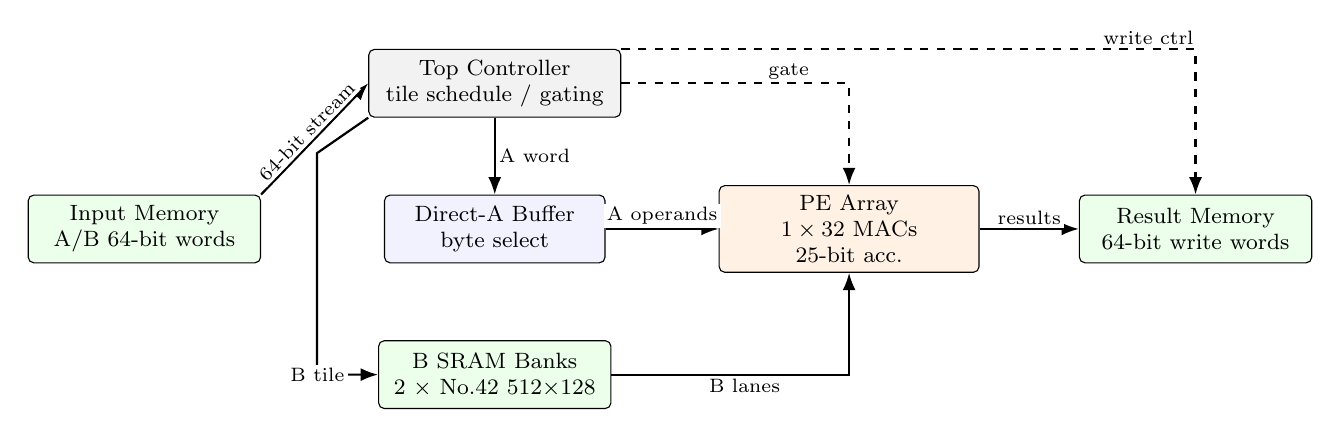
\begin{tikzpicture}[
  font=\footnotesize,
  block/.style={draw, rounded corners=2pt, minimum width=2.8cm, minimum height=0.86cm, align=center, fill=blue!5},
  mem/.style={draw, rounded corners=2pt, minimum width=2.95cm, minimum height=0.86cm, align=center, fill=green!8},
  core/.style={draw, rounded corners=2pt, minimum width=3.3cm, minimum height=1.1cm, align=center, fill=orange!10},
  ctrl/.style={draw, rounded corners=2pt, minimum width=3.2cm, minimum height=0.86cm, align=center, fill=gray!10},
  note/.style={font=\scriptsize, fill=white, inner sep=1.2pt, align=center},
  arr/.style={-{Latex[length=2.2mm]}, thick},
  dashedarr/.style={-{Latex[length=2.2mm]}, thick, dashed}
]
  \node[mem] at (0,0) (input) {Input Memory\\A/B 64-bit words};
  \node[ctrl] at (4.45,1.85) (ctrl) {Top Controller\\tile schedule / gating};
  \node[block] at (4.45,0) (abuf) {Direct-A Buffer\\byte select};
  \node[mem] at (4.45,-1.85) (bsram) {B SRAM Banks\\2 $\times$ No.42 512$\times$128};
  \node[core] at (8.95,0) (pe) {PE Array\\$1\times32$ MACs\\25-bit acc.};
  \node[mem] at (13.35,0) (result) {Result Memory\\64-bit write words};

  \draw[arr] (input.north east) -- node[note, above, sloped] {64-bit stream} (ctrl.west);
  \draw[arr] (ctrl.south) -- node[note, right] {A word} (abuf.north);
  \draw[arr] (ctrl.south west) -- ++(-0.65,-0.45) |- node[note, pos=0.76, left] {B tile} (bsram.west);
  \draw[arr] (abuf.east) -- node[note, above] {A operands} (pe.west);
  \draw[arr] (bsram.east) -| node[note, pos=0.28, below] {B lanes} (pe.south);
  \draw[arr] (pe.east) -- node[note, above] {results} (result.west);
  \draw[dashedarr] (ctrl.east) -- ++(1.15,0) -| node[note, pos=0.28, above] {gate} (pe.north);
  \draw[dashedarr] (ctrl.north east) -- ++(5.3,0) -| node[note, pos=0.35, above] {write ctrl} (result.north);
\end{tikzpicture}
}
\caption{最终加速器结构与数据流向}
\end{figure}

\begin{table}[H]
\centering
\caption{最终 RTL 参数}
\begin{tabular}{lll}
\toprule
参数 & 数值 & 说明 \\
\midrule
\texttt{MATRIX\_SIZE} & 512 & 矩阵维度 \\
\texttt{TILE\_ROWS} & 1 & 每个 compute tile 的 A 行数 \\
\texttt{TILE\_COLS} & 32 & 每个 compute tile 的 B 列数 \\
\texttt{B\_BANKS} & 2 & B SRAM bank 数量 \\
\texttt{ACC\_BITS} & 25 & PE 内部累加器位宽 \\
结果输出位宽 & 32 bit & 写回时符号扩展为 32 bit \\
SRAM macro & No.42 \texttt{512x128} & B tile 存储使用两个 bank \\
时钟约束 & 10.00 ns & 单时钟，100 MHz 功耗评估 \\
\bottomrule
\end{tabular}
\end{table}

选择 $1\times32$ 的原因是它在固定 PE 数较小的情况下减少 column tile 数，并能充分使用两个 128 bit B SRAM bank。A 侧直接使用 64 bit input word buffer，避免在 PPA 口径中引入额外 A SRAM macro。

\section{主要优化方法}

\subsection{Direct-A 与 B tile 复用}

A 矩阵按 64 bit word 读取，每个 word 包含 8 个 SINT8 元素。controller 将 A word 保存在寄存器 buffer 中，并逐 byte 提供给计算核。B 矩阵按 column tile 预先装入两个 \texttt{512x128} SRAM bank，之后在该 column tile 内跨所有 row tile 复用，从而降低 B 载入开销。

\subsection{A-zero 稀疏门控}

输入数据具有较多零值。最终版本在 controller 中检测当前 A byte：当 A byte 为 0 时，不发出 PE pulse，同时关闭对应 B SRAM read/prefetch 的 chip-select。logic-only 综合顶层中也使用 \texttt{pulse\_en \&\& (a\_sram\_rdata != 0)} 作为计算核使能，使门控在综合 PPA 中可见。

\subsection{PE 操作数隔离}

PE 内部在 \texttt{pulse\_en=0} 时将乘法器 A/B 输入置零，仅在有效 pulse 时更新累加器。该结构降低无效周期的切换活动，并保持累加结果不变。

\subsection{计算地址气泡消除}

行为级 SRAM 为同步读。早期版本每个 A word 计算前需要一个 \texttt{S\_COMPUTE\_ADDR} 读地址气泡。最终版本在 \texttt{S\_LOAD\_A\_WRITE} 的最后一行同时发出第一个 B SRAM read，使下一拍可以直接进入 \texttt{S\_COMPUTE\_PULSE}，减少每个 A word 的空拍。

\subsection{结果写回流式化}

原始结果写回采用 setup/hold 两拍写一个 64 bit word。最终版本保留第一个 setup 拍，之后在 \texttt{S\_WRITE\_HOLD} 中每拍写出上一个已稳定 word，同时准备下一个 word 的地址和数据。最后一个 word 通过同步 result RAM 的下一拍写入完成 flush。该优化不改变 logic-only 计算核 PPA，但将完整 pre-syn 周期数降至 5,464,066。

\subsection{低漏电综合策略}

综合脚本使用 logic-only 顶层 \texttt{accelerator\_logic\_top}，时钟周期设为 \SI{10.00}{ns}，并采用
\begin{verbatim}
compile_ultra -gate_clock -area_high_effort_script
\end{verbatim}
该策略在满足 timing 的同时降低 cell area 和 leakage。综合脚本显式排除 SRAM macro、controller 和外部 memory，符合 PPA 统计要求。

\section{验证流程}
在远端clab环境跑完整流程：
\begin{enumerate}
  \item pre-syn VCS 跑功能仿真并生成 \texttt{result\_mem.csv}；
  \item 将 \texttt{result\_mem.csv} 抓回本地，在 Python venv 中运行 \texttt{CheckResult.py}；
  \item Design Compiler 跑 logic-only 综合并生成 area/power/timing report、门级网表和 SDF。
\end{enumerate}

验证输出如下：
\begin{itemize}
  \item Pre-syn VCS: \texttt{[TB][LATENCY] cycles=5464066 realtime\_ns=5464066.500}
  \item Checker: \texttt{Correct!}, \texttt{loss=0}, \texttt{relative\_loss=0.0}, \texttt{sse=0.0}
\end{itemize}

\section{最终 PPA 结果}

\subsection{延迟}

DC target clock 为 \SI{10.00}{ns}，最差 setup slack 为 \SI{9641.00}{ps}，因此 shortest-period basis 为
\begin{equation}
  T_{\mathrm{short}} = 10000\ \mathrm{ps} - 9641.00\ \mathrm{ps} = 359.00\ \mathrm{ps}.
\end{equation}
完整功能仿真周期数为 5,464,066，因此
\begin{equation}
  L = 5{,}464{,}066 \times 0.359\ \mathrm{ns} = 1{,}961{,}599.694\ \mathrm{ns}.
\end{equation}

\subsection{逻辑综合结果}

\begin{table}[htbp]
\centering
\caption{Design Compiler logic-only 结果}
\begin{tabular}{lr}
\toprule
项目 & 数值 \\
\midrule
Total cell area & $4296.081454\ \mu m^2$ \\
Total dynamic power & $0.3437407\ \mathrm{mW}$ \\
Cell leakage power & $5.0590\ \mathrm{mW}$ \\
Logic total power & $5.4027407\ \mathrm{mW}$ \\
Worst setup slack & $9641.00\ \mathrm{ps}$ \\
\bottomrule
\end{tabular}
\end{table}

\subsection{SRAM 功耗统计}

选用两个 No.42 \texttt{512x128} SRAM macro。单个 macro 在 100 MHz 下 dynamic power 为 $0.08043\ \mathrm{mW}$，leakage 为 $0.05155885\ \mathrm{mW}$。A-zero 门控后，B SRAM active cycles 为
\begin{equation}
  169{,}336\times16 + 16\times512 = 2{,}717{,}568.
\end{equation}
总周期数为 5,464,066，因此 B SRAM duty 为
\begin{equation}
  \frac{2{,}717{,}568}{5{,}464{,}066} = 49.735270\%.
\end{equation}
最终 sparse-aware SRAM power 为 $0.183121856\ \mathrm{mW}$。

\subsection{总结果}

最终指标为 SSE、latency 和 power 三项。SSE 由 checker 对输出矩阵和参考矩阵逐元素求平方误差得到：
\begin{equation}
  \mathrm{SSE}=\sum_{i,j}\left(C_{\mathrm{out}}(i,j)-C_{\mathrm{ref}}(i,j)\right)^2=0.
\end{equation}

Latency 使用功能仿真周期数和 DC timing 得到的 shortest-period basis 计算：
\begin{equation}
  \mathrm{Latency}=5{,}464{,}066\times(10{,}000-9{,}641)\ \mathrm{ps}
  =1{,}961{,}599.694\ \mathrm{ns}.
\end{equation}

Power 采用 logic-only 综合功耗加 sparse-aware SRAM 功耗。逻辑功耗为
\begin{equation}
  P_{\mathrm{logic}}=0.3437407+5.0590=5.4027407\ \mathrm{mW}.
\end{equation}
两个 B SRAM 的 duty 为 $2{,}717{,}568/5{,}464{,}066=49.735270\%$，因此
\begin{equation}
  P_{\mathrm{SRAM}}=2\times\left(0.05155885+0.08043\times0.49735270\right)
  =0.183121856\ \mathrm{mW}.
\end{equation}
最终总功耗为
\begin{equation}
  P_{\mathrm{total}}=5.4027407+0.183121856=5.585862556\ \mathrm{mW}
  =5{,}585{,}862{,}556\ \mathrm{pW}.
\end{equation}

\begin{table}[htbp]
\centering
\caption{最终结果汇总}
\begin{tabular}{lr}
\toprule
项目 & 数值 \\
\midrule
SSE & 0 \\
Latency & $1{,}961{,}599.694\ \mathrm{ns}$ \\
Power & $5{,}585{,}862{,}556\ \mathrm{pW}$ \\
\bottomrule
\end{tabular}
\end{table}

\section{结论}

最终版本在保持 $\mathrm{SSE}=0$ 的前提下，采用 direct-A $1\times32$ 计算结构、两个 \texttt{512x128} B SRAM bank、A-zero 稀疏门控、PE 操作数隔离、计算地址气泡消除和结果写回流式化。完整远端验证通过，最终 latency 为 $1{,}961{,}599.694\ \mathrm{ns}$，总 sparse-aware power 为 $5{,}585{,}862{,}556\ \mathrm{pW}$。

\end{document}